\chapter{基于国产AI处理器的Top-k算法性能优化}


本章首先介绍了阿姆达尔定律和古斯塔夫森定律,为Top-k算子的性能优化指明了方向,即提升Top-k算子程序的并行度。接着从计算效率方面入手,充分利用国产AI处理器支持多级并行计算的优势,提高了Top-k算子的并行计算能力。最后从访存效率角度出发,通过多种优化技巧减少了Top-k算子的访存耗时。

\section{算子优化策略}

阿姆达尔定律是计算机科学领域的一条经验定律,该定律表明了并行计算、存储系统获得的加速比和处理器数量以及程序并行化程度之间的关系,其计算公式见(4.1)。

\begin{equation}
S = \frac{1}{1 - P + \frac{P}{N}}
\label{eq:4.1}
\end{equation}

式(4.1)中,$S$表示并行化前后程序获得的加速比,$P$表示程序中可实现并行化处理部分的比例,$N$则表示并行处理器的数量。从该式可以看出,当$P$不变时,程序用到的并行处理器数量越多,就能获得越大的加速比。但是当$N$远大于$P$时,程序获得的加速比会逐渐趋近于固定的数值。即当$N$趋近于无穷大时,式(4.1)近似为(4.2)。

\begin{equation}
S = \frac{1}{1 - P}
\label{eq:4.2}
\end{equation}

式(4.2)表明即使处理器数量足够的多,倘若程序并行化处理代码占比不高的话,那么程序依然无法获得很好的加速比。因此要想获得更大的加速比,这就需要开发者充分发掘程序中可进行并行化处理的部分,从而尽量提升程序中并行化处理代码的占比。

根据阿姆达尔定律,在处理器足够多的条件下,当程序并行化处理比例达到95\%时,程序获得的加速比也依然只有20倍。这是因为阿姆达尔定律限定了处理问题的规模以及程序可并行化的比例。在实际中通常使用大量的处理器来处理大规模的问题,这些大规模的问题也能分成多个小规模的问题进行并行处理。在这样的背景下,古斯塔夫森定律被提出,其公式见(4.3)。

\begin{equation}
S = N - P \cdot (N - 1)
\label{eq:4.3}
\end{equation}

式(4.3)中,$S$表示并行化前后程序获得的加速比,$N$表示并行处理器的数量,$F$表示程序中串行部分代码的占比。该式表明,当程序的串行部分代码占比足够小,即程序并行化程度足够大时,程序获得的加速比和处理器数量成正比。因此在程序并行化程度足够高的情况下,增加处理器数量可以很好地提升程序运行的性能。
通过上述两个定律可知,在处理器数量不变的条件下,若想对实现的Top-k算子子程序进行性能调优,就需要尽可能地提升算子代码的并行化程度。根据MLU系列AI处理器的硬件架构特性,可以从计算效率和访存效率两个方面提高算子程序的并行度。


\section{Top-k算法访存效率优化}
% \subsection{radix-select Top-k 算法的digit调优}

% 以float-int32+默认kernel作为一般情况分析:radix的选择(对应代码变量
% digit的大小),当digit为1的时候,bucket\_num=2,float对应32bit,需要32次捞取,digit为4,bucket\_num=16,
% 需要8次捞取,digit为32,bucket\_num=2\^32,需要捞取1次,radix选择的越大,
% 则总的I/O时间越短。



\subsection{显存I/O优化}
在国产 AI 处理器的复杂体系结构中,显存 I/O 操作的效率是制约整体系统性能提升的关键因素
之一。数据双缓冲、数据对齐以及数据缓存作为重要的优化策略,从不同角度对显存 I/O 进行精细
化调控,旨在最大程度地提高数据传输速率、降低延迟并提升资源利用率,以满足国产 AI 处理器
在多样化人工智能任务中的严苛需求,增强其在全球 AI 计算领域的竞争力与适应性。


\paragraph{数据对齐优化分析}

显存带宽利用率是指在国产AI处理器中,实际使用的显存带宽与显存理论带宽的比率。
显存带宽是指显存与 核心之间数据传输的速率,
它的计算公式为:带宽 = 显存频率 × 显存位宽 ÷8(单位为字节 / 秒)。
例如,一款显存频率为 1000MHz、显存位宽为 128 位的显卡,
其理论带宽为 1000MHz×128÷8 = 16000MB/s。
显存带宽利用率优化的目的是尽可能地提高这个比率,使显存与片上内存(或寄存器)之间的数
据传输更加高效,从而提升整个系统的性能。
针对国产AI处理器,常用的优化方法包括数据布局优化。

a.连续内存访问:在BangC编程中,应该尽可能地保证数据在显存中的存储是连续的。
因为在访问连续内存时,缓存命中率更高,数据传输效率也更高。
对于MLU-Core内的访存行为而言,其主要针对NRAM空间,在数据到达NRAM空间后,数据已经是连续存储。
但对于MLU-Core针对GDR进行访问时,MLU-Core之间的不连续的访问模式将可能会导致GDR的bank冲突。
而所谓bank冲突即:
GDR被划分为多个bank(优点是可以隐藏部分延时),GDR的吞吐是建立在bank负载均衡的前提下,如果有多个请求同时落在
同一个Bank内,那它一次只能响应其中一个,导致这些请求会被序列化,这就是Bank Conflict(Bank冲突)。
发生 冲突的bank负载是满的,问题是其他bank的请求是不足的,也就是负载不均衡,导致带宽利用率不足。
bank冲突和请求的地址,GDR的形态以及地址映射相关。
在国产AI处理器上是 5HBM × 8 channel * 32KB=1.25MB。通过MLU-Core间连续访存可以有效的规避Bank冲突。
主要通过更改task与数据之间的映射关系即可实现。参考下图~\ref{fig:bank_conflic}:

\begin{figure}[ht]
    \centering
 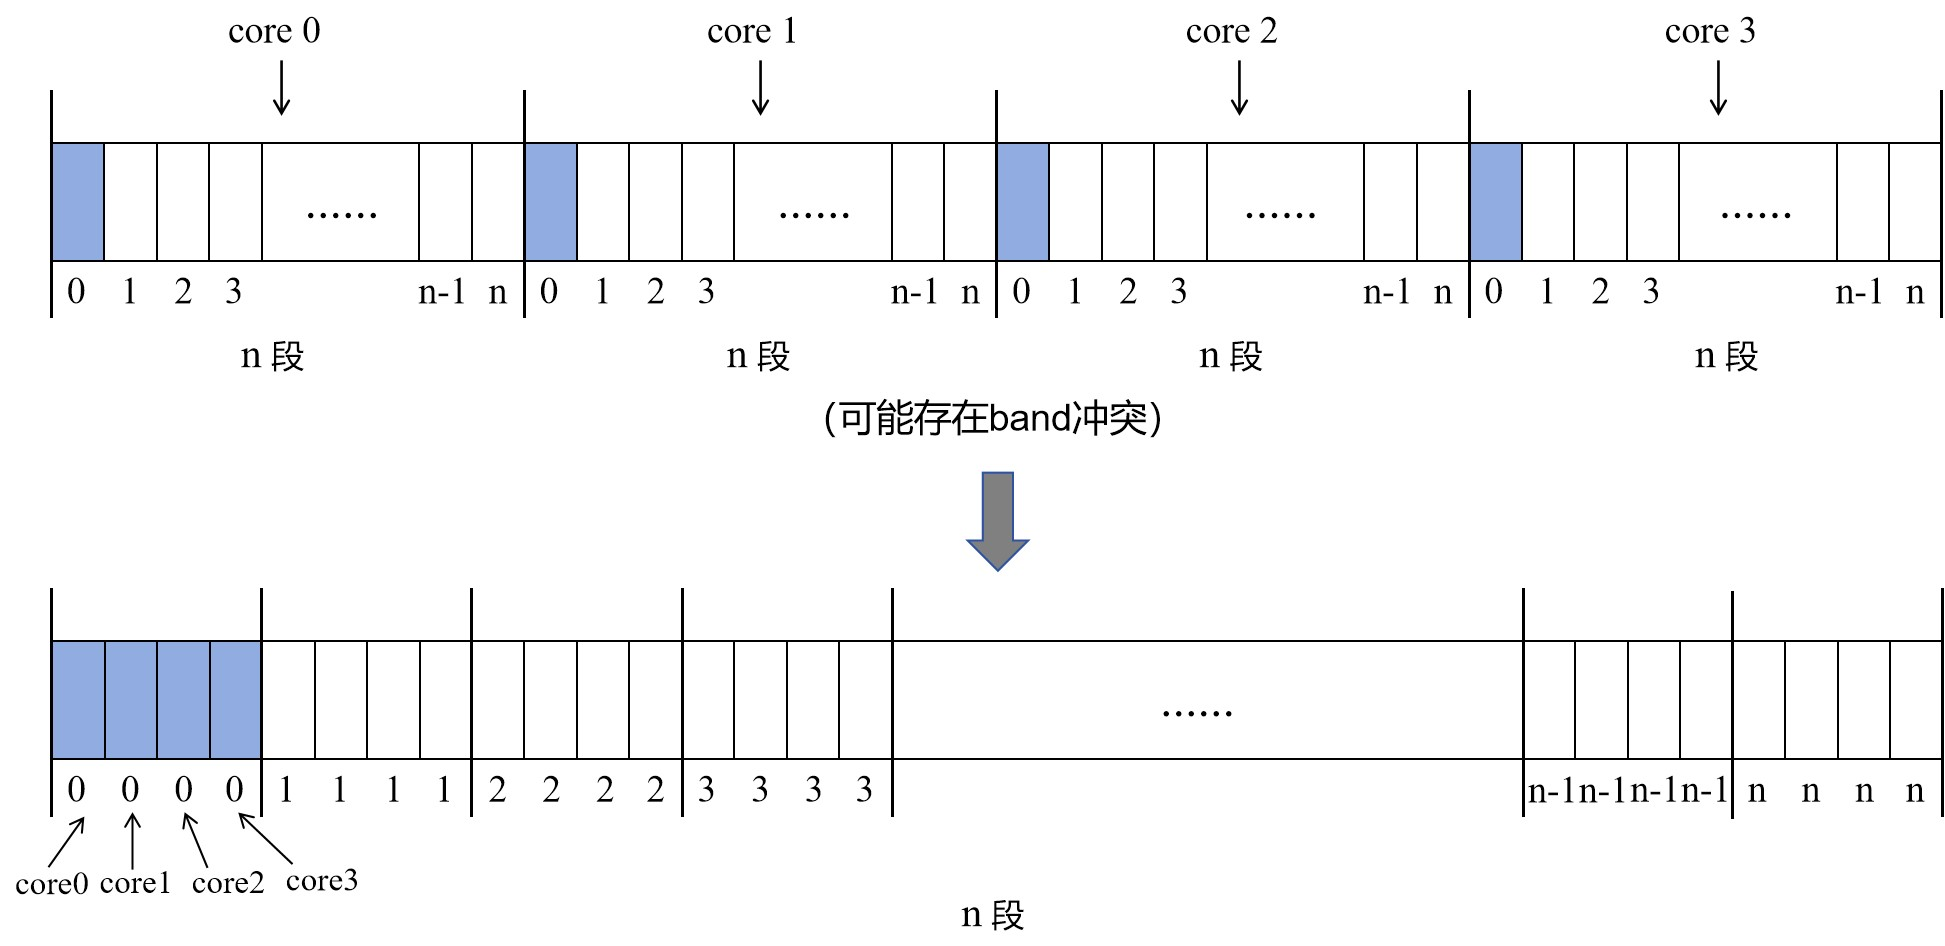
\includegraphics[width = 0.9\textwidth]{bank_conflic_1.jpg}
    \caption{Cluster级连续I/O示意图}
    \label{fig:bank_conflic}
    % \note{注:图注的内容不宜放到图题中。}
\end{figure}





b.数据对齐:确保数据的存储地址按照 的内存访问要求进行对齐。不同的 架构对内存对齐有不
同的要求,一般来说,将数据的起始地址对齐到缓存行大小(如 32 字节或 64 字节)的倍数,
可以提高内存访问效率。对于国产AI处理器的不同层次的内存,其对齐要求见下
表~\ref{tab:alignment}。

\begin{table}
    \caption{存储类型及其对齐方式}
    \centering
    \begin{tabular}{lcc}
    \toprule
    存储类型 & 地址对齐 & 数据对齐 \\
    \midrule
    NRAM & 16B & 128B \\
    SRAM & 16B & 128B \\
    WRAM & 64B & 128B \\
    GDRAM & 512B & 512B \\
    LDRAM & 512B & 512B \\
    \bottomrule
    \end{tabular}

    \label{tab:alignment}
    \end{table}
此优化方法体现在对各个变量进行空间划分时,大小尽可能满足数据对齐的倍数即可。


\paragraph{双缓冲优化分析}

数据双缓冲机制基于并行处理思想,于国产 AI 处理器与显存间构建缓冲 A 和缓冲 B 两个独立缓冲区。数据传输时,缓冲 A 数据被处理,缓冲 B 可填充,反之亦然。设数据处理时间为\(T_{\text{process}}\),数据填充时间为\(T_{\text{fill}}\),传统单缓冲总时间\(T_{\text{single}} = T_{\text{process}} + T_{\text{fill}}\),双缓冲总时间\(T_{\text{double}}=\max(T_{\text{process}}, T_{\text{fill}})\),该并行模式减少数据等待时间,提升数据传输效率与显存 I/O 吞吐率。
在国产AI处理器显存与计算单元中间,存在多级的内存层次。其中共享内存和NRAM可以通过程序来进行
访存行为的控制。因此可以基于这一点将双缓冲优化手段应用于Top-k算子的开发过程中。
对于Top-k算子而言,其filter阶段可以运行流水机制。
同时,MLU Core 支持多指令流并行,Topk 算子各计算阶段涉及加载输入数据、计算输入数据
和存储计算结果。加载与存储指令分配到数据搬移队列,计算指令分配到数据计算队列。
有数据依赖的计算与访存指令时序分开,无依赖的则并发执行,减少指令等待时间,提高访存效率
,提升 Top-k 算子性能,此计算与访存并行通过软流水实现。软流水是特殊指令重排,将同一
循环内不同循环迭代间计算和访存重组,使处理同一批数据的计算和访存分散到不同循环迭代,
消除同一循环迭代内计算与访存依赖关系,让指令并行执行,相互隐藏执行时间,减少循环体总
执行时间,后续将阐述 Top-k 算子访存效率优化中的三级流水和五级流水机制。


\subparagraph{三级流水}
常用的三级流水,如图~\ref{fig:three_level}所示。其中L代表Load操作,表示将数据从GDRAM或者SRAM加载到NRAM的过程;C代表Compute,表示数据在MLU Core上运算的过程;S代表Store操作,表示将计算结果从NRAM存回到GDRAM或者SRAM的过程。在空间维度上,片上空间被划分为Ping和Pong两块,每块都可以用来临时存放输入数据和输出数据;在时间片维度上,可进行的访存或计算操作包括了Load,Compute和Store。
\begin{figure}[ht]
    \centering
    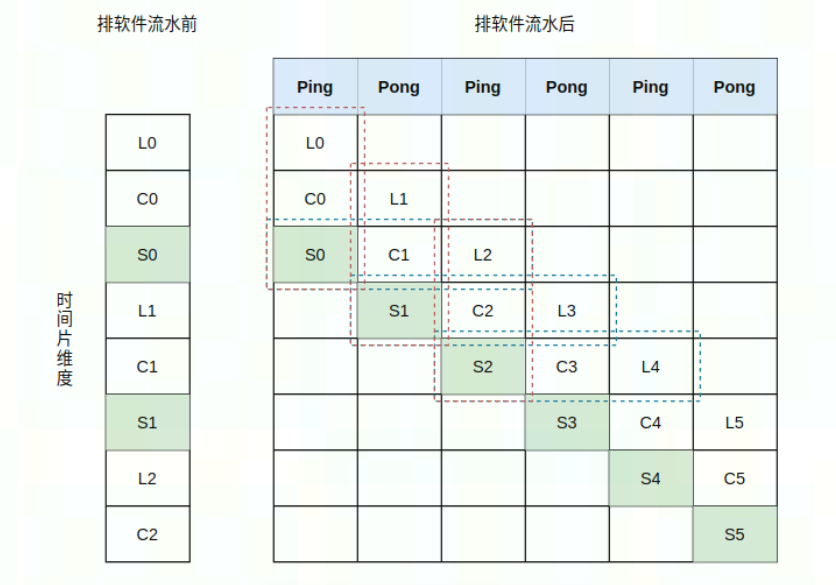
\includegraphics[scale = 0.5]{three_level.png}
    \caption{三级流水示意图}
    \label{fig:three_level}
    % \note{注:图注的内容不宜放到图题中。}
\end{figure}
从图~\ref{fig:three_level}可知,通过软流水,在同一个时间片内可以进行加载(Load)、计算(Compute)以及存储(Store)操作。当MLU核心进行计算操作时,各个存储空间也在不断地进行数据传输操作,从而实现了计算与访存的并行,减少了数据等待时间,进而提高了访存效率。

需要注意的是,由于片上随机存取存储器(NRAM)的容量有限,对于计算过程较为复杂的计算任务,通常会将NRAM划分成多段。
若再进行乒乓分区,MLU核心一次能处理的数据量将会进一步减少。
在这种情况下,软流水往往会带来负面效果。因此,仅对于过滤(FILTER)阶段的计算,进行三级流水操作。


\subparagraph{五级流水}

五级流水是在三级流水的基础上,利用硬件内存核心(Memory Core)实现的。它以静态随机存取存储器(SRAM)作为缓冲区,
将加载(Load)和存储(Store)操作各分为两部分,一部分由MLU核心完成,另一部分由内存核心(Memory Core)完成。
在Top-k算子的过滤(FILTER)计算阶段,可以利用SRAM来完成结果的缓存。实际上,SRAM也可用于对整个计算过程实现五级软流水操作。
整个五级流水过程如下:
首先由 Memory Core 将数据从 GDRAM 搬运到 SRAM 中,然后再由 coreDim(以 4 为例)个 MLU-Core 分别从 
SRAM 搬运部分数据到 NRAM 中进行计算,计算结果先由 coreDim 个 MLU Core 搬运到 SRAM 上,再由 Memory Core 从 
SRAM 搬运到 GDRAM 上。五级 软件流水运行过程,
如图~\ref{fig:five_level} 所示。
\begin{figure}[ht]
    \centering
    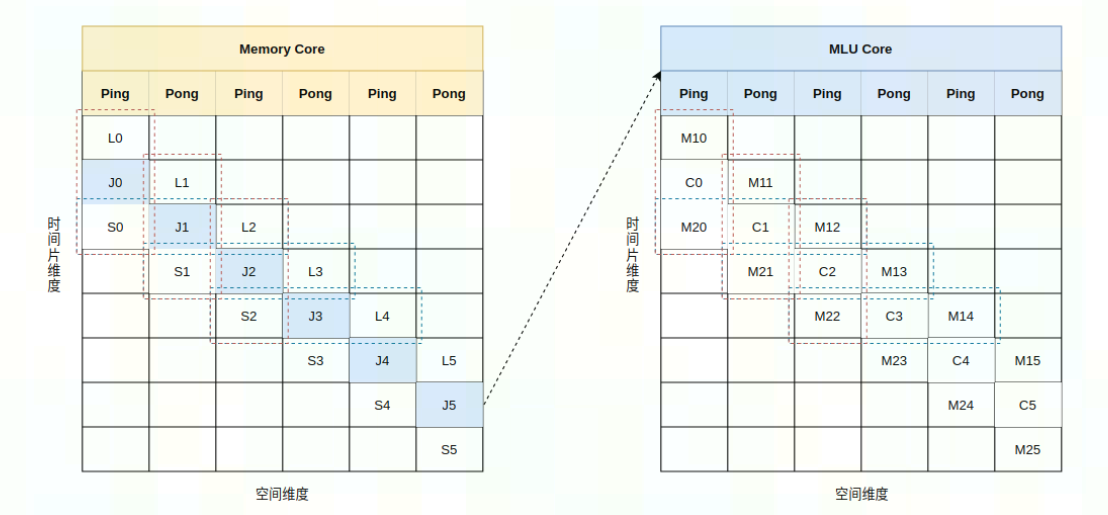
\includegraphics[scale = 0.5]{five_level.png}
    \caption{五级流水示意图}
    \label{fig:five_level}
    % \note{注:图注的内容不宜放到图题中。}
\end{figure}
在空间维度上,片上空间 SRAM 和 NRAM 都被划分为 Ping 和 Pong 两块, 每块都可以用来临时存放输入向量和输出向量;
在时间片维度上,Memory Core逻辑可以分为三部分: Load、Job(MLU Core 处理)和 Store;
MLU Core 逻辑也分 为三部分:Move1、Compute 和 Move2。从 MLU Core 的角度来看,
M1->C->M2 构 成了三级流水,从由 Memory Core 的角度来看,五级流水就可以理解成 L->MLU Core->S 的三级流水。
以 L0->J0->S0 为例,当 L0 将数据从 GDRAM 搬运到 SRAM上以后,通过 MLU Core 的三级流水处理将结果保存到 SRAM 上,
然后由 S0 将 结果搬运到 GDRAM 上。






\section{Top-k算法计算效率优化}
基于 MLU 系列 AI 处理器的并行计算系统支持服务器级、板卡级、芯片级、Cluster 级、MLU Core 级、指令级以及数据级共七个级别的并行计算。
Top-k 算 子计算效率优化的过程,就是将其计算任务映射到不同的并行层次的过程。服务 器级和板卡级的并行计算通常是面向 AI 训练和大规模推理任务,
通过调用 CL(Communications Library,通信库)和 RT(Runtime Library,运行时库)接口实 现。而其他层级的并行计算能力则是可以通过 BC 语言编程实现。
例如在上个章 节中设计实现的 Top-k 算子,通过使用 BC 智能编程语言提供的向量化操作指令, 对计算数据进行向量化处理,大大减少了整个算法过程需要执行的指令数量和
 循环迭代次数,从而提升 Top-k 特征向量的求取速度,这属于数据级并行计算。 指令级并行更多是通过提升访存效率来实现对算子的整体性能优化,对计算效 率提升较为有限,
 因此可将其结合到 MLU Core 级并行优化方案中一同进行。综 上所述。接下来将从 MLU Core 级并行、Cluster 级并行以及芯片级方面入手,来 进行 Top-k 算子的计算
 效率优化工作。

\subsection{Core级优化}

\paragraph{算法优化}
对于RadixSelect算法而言,在特定的情况下,数据可能会落入所有的桶中,这将会使得
FILTER阶段的操作变得没有意义,因为此时不存在无效数据。因此在FIND TARGET BUCKET阶段,
可以对各个桶进行检查:当桶中的数据等于本轮迭代所有数据个数时,直接进入到下一次迭代。
这将有效的减少冗余计算。更改后的FIND TARGET BUCKET阶段伪代码片段如下:
% \begin{algorithm}
%     \tcp{\underline{FIND TARGET BUCKET}\; }
%     \For{$i \leftarrow 0$ to $2^r - 1$}{
%         \If{$Bucket[i] \eq AllNum$}{
            
%             \textbf{break}\;
%         }\\
%         \If{$Bucket[i] \ge k$}{
%             $POS \leftarrow Bucket[i]$\;\\
%             \textbf{break}\;
%         }
%     }
%     % \caption{CountingSort Algorithm-Early Stop}
% \end{algorithm}

\begin{algorithm}
    \caption{CountingSort Algorithm-Early Stop}
    \label{alg:counting_sort_early_stop}
    \tcp{\underline{FIND TARGET BUCKET WITH EARLY STOP}\; }
    $STOP \leftarrow False$\\
    \For{$i \leftarrow 0$ to $2^r - 1$}{
        \If{$Bucket[i] = AllNum$}{
            $STOP \leftarrow True$\\
            \textbf{break}\;
        }    
        \If{$Bucket[i] \ge k$}{
            $POS \leftarrow Bucket[i]$\;\\
            \textbf{break}\;
        }
    }
    \If{$STOP = True$}{
        \textbf{break}\;
    }
\end{algorithm}
% 整体伪代码如下:
% \begin{algorithm}
%     \SetAlgoNoLine 
%     % \SetAlgoLined
%     % \LinesNumbered            % 强制显示所有行号
%     \KwIn{Array $D$ with $n$ entries, integer $k \leq n$}
%     \KwOut{array R is the Top-k elements}
%     $Bucket \leftarrow$ init $0$ \tcp{Initialize buckets}
%     \tcp{\underline{HISTOGRAM - KEYS}\; }
%     \For{$j \leftarrow 0$ to $N - 1$}{
%         $Bucket[D[j]] \leftarrow Bucket[D[j]] + 1$
%     }
%     \tcp{\underline{SCAN - BUCKETS}\; }
%     $Sum \leftarrow 0$\;\\
%     \For{$i \leftarrow 0$ to $2^r - 1$}{
%         $Val \leftarrow Bucket[i]$\\
%         $Bucket[i] \leftarrow Sum$\\
%         $Sum \leftarrow Sum + Val$
%     }
%     \tcp{\underline{FIND TARGET BUCKET WITH EARLY STOP}\; }
%     $STOP \leftarrow False$\\
%     \For{$i \leftarrow 0$ to $2^r - 1$}{
%         \If{$Bucket[i] = AllNum$}{
%             $STOP \leftarrow True$\\
%             \textbf{break}\;
%         }    
%         \If{$Bucket[i] \ge k$}{
%             $POS \leftarrow Bucket[i]$\;\\
%             \textbf{break}\;
%         }
%     }
%     \If{$STOP = True$}{
%         \textbf{break}\;
%     }

%     \tcp{\underline{FILTER}\; }
%     \For{$j \leftarrow 0$ to $N - 1$}{
%         \If{$D[j] \ge POS$}{
%             \textbf{continue}\;
%         }
%         $A \leftarrow Bucket[D[j]]$\\
%         $R[A] \leftarrow K[j]$\\
%         $Bucket[D[j]] \leftarrow A + 1$
%     }
%     \caption{CountingSort Algorithm}
% \end{algorithm}
\paragraph{预处理计算优化}
    对于Top-k算子而言,RadixSelect算法仅将Top-k 大/小的值筛选出来。对于内部排序
    还需要根据sorted参数来决定是否使用RadixSort算子进行计算。
    而正负性等数值特性对于RadixSort和RadixSelect的影响是相同的,
    因此通过将RadixSelect和RadixSort的
    预处理方式进行对齐,能够有效的减少指令数目,提高Top-k算子的计算效率。

    通过前文的分析,我们总结出RadixSort和RadixSelect预处理方案如下:
    \begin{enumerate}
        \item Top-k小,整型,所有数的符号位进行取反操作。
        \item Top-k小,浮点型,对正数进行符号位取反,对负数全部 bit 位进行取反,
        即非负数与 0x80000000 进行位异或操作, 负数与 0xffffffff 进行位异或操作
        \item Top-k大,整型,对所有数据的非符号位实施取反操作。
        \item Top-k大,浮点型,数据的符号位保持不变且负数无需进行任何改动,
        对非负数的非符号位进行取反操作。
    \end{enumerate}

    而后,根据sorted参数来判断是否需要运行RadixSort核函数。若是需要运行,此时RadixSelct
    的输出不需要进行后处理,直接将其作为RadixSort的输入即可。



\paragraph{指令流水线优化}
MLU-Core 内具有多条独立执行的指令流水线(以下简称为 PIPE),分别 为负责标量运算的 ALU-PIPE、负责向量运算的VFU-PIPE、
负责张量运算的TFU-PIPE、负责片上和片外数据搬移的 IO-DMA\ PIPE 和负责片上数据搬移的Move-DMA PIPE。如图~\ref{fig:inst_queue}所示,
Inst-Cache 中的一段指令序列顺序开始执行后, 经过分发和调度被分配进了多个 PIPE 队列中,进入 PIPE 前指令是按顺序执行 译码的,而进
入不同计算或访存队列后则由硬件解决寄存器重命名或读写依赖。 这意味着不同计算或者访存类型指令是可以并行执行的。
例如每次迭代的开始,需要用到 bang\_write\_value 指令对Buckets数组进行初始化。
而在bang\_write\_value指令 Compute 流执行,同样可实现给指定内存段赋 初值的
 memset\_nram 指令则在 Move 流执行。因此通过使用 memset\_nram 指令替代
 bang\_write\_value,可以实现向量运算与内存段赋初值操作并行执行,
 减少总的指令运行耗时。
\begin{figure}[ht]
    \centering
    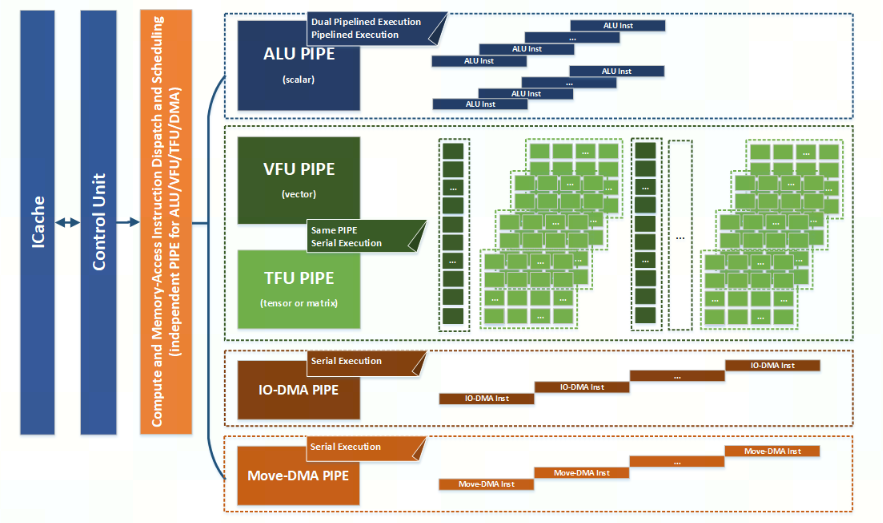
\includegraphics[scale = 0.5]{inst_queue.png}
    \caption{多队列指令流水线}
    \label{fig:inst_queue}
    % \note{注:图注的内容不宜放到图题中。}
\end{figure}

\paragraph{指令融合优化}
BC 编程语言还提供了多个指令融合操作接口,这类接 口不仅可以减少数据中转和 NRAM 空间
占用,还可以利用硬件的指令融合功能 达到更高的性能。在整个 Top-k 算子的计算流程中,
先后多次使用了bang\_mul、bang\_add 和 bang\_sub 等向量操作指令。
通过使用bang\_fusion 指令融合接 口,可以实现三个输入向量的乘加、乘减、加乘、
减乘、减减、加加、加减、减加运 算。从而进一步减少计算过程中用到的指令数量,提升算
子的性能。如图~\ref{fig:fusion}所 示,使用融合指令替换原指令组合后,可以在一条指令时间内完成乘
加操作。在RadixSelect实现阶段,数据预处理阶段满足指令融合的要求,因此在此阶段可以进行指令融合。
\begin{figure}[ht]
    \centering
    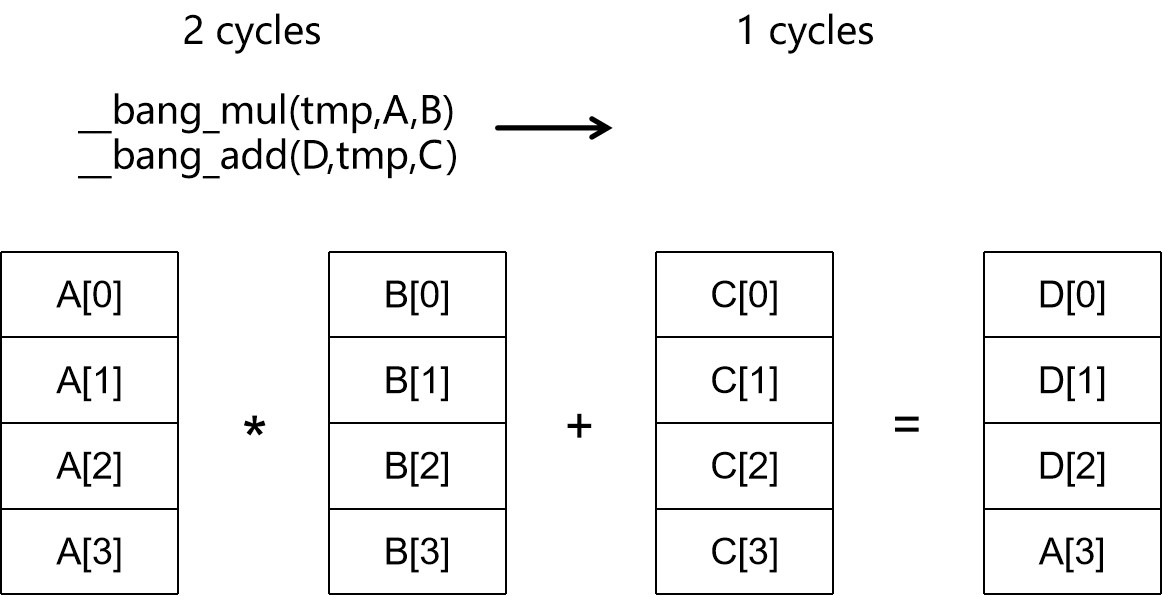
\includegraphics[scale = 0.47]{fusion.jpg}
    \caption{指令融合示例图}
    \label{fig:fusion}
    % \note{注:图注的内容不宜放到图题中。}
\end{figure}



\subsection{Cluster级优化}
MTP Cluster 架构如图~\ref{fig:cluster_arch}所示,MTP Cluster 由 4 个 MLU Core 和一个 Memory Core 组成,
是 MTP 架构中的最小执行单元。每个 MLU Core 是具备完整计算、IO 和控制功能的处理器核心,
可以独立完成一个计算任务,也可以与其他 MLU Core 协作完成一个计算任务。
而任务类型描述的是任务的硬件需求,任务规模描述的是任务的划分方式,而任务映射则建立了具体任务与物理硬件之间的映射关系。
为了便于描述任务规模,在BANG C 编程语言中引入了cnrtDim3\_t 数据类型。
其中,与任务规模相关的内置变量包括: taskDim 、 taskDimX 、 taskDimY 以及 taskDimZ。
对于 UnionN 类型的任务,需要至少有 N 个 Cluster 空闲时才能下发任务。
同时还要满足约束 taskDimX \% (N * coreDim) = 0 。最小的并行度为 clusterDim * coreDim 。
在不考虑任务展开的情况下,迭代次数=taskDimZ * taskDimY * taskDimX / (N * coreDim) 。
驱动根据当前硬件的实时利用率决定是否将任务展开,尽可能占满所有的硬件资源。
例如:当任务类型为Union1, 任务规模为 {X=8, Y=1, Z=1} 时,默认情况下,
该任务会在一个Cluster上经过两轮迭代才成完成。
如果,驱动在下发任务时发现硬件至少有两个Cluster空闲,那么还会做任务展开,
让Union1类型的任务同时占用2个Cluster,这样只需要一轮迭代即可完成。

在定义Job类型为UnionX类型时,Job被调度的物理单元将会以X个Cluster为单位。通过前文的介绍,
我们知道RadixSelect核函数的Job数量由A来确定,即每个Job处理输入的一行,因此将会有A个Job。
具体的Job类型由B的大小来确定,或者说单个Job所占的硬件资源由B确定。

因此,若是按照上述固定的规则
但是当A的数量较少,B的数值很大时,将会出现某些MLU-Core不满足Job的构成规则而处于闲置的状态。
例如,假如芯片上有24个Cluster(96个MLU-Core), 并且此时的A数值为9,B数值同样很大(大于200w),此时Job类型将会被定义
为Union4类型,即单个Job将会占据16个Cluster(64个MLU-Core),剩下的8个将会一直处于闲置状态,
Cluster的利用率为75\%。而假若此时设定为Union3类型,则对于整个计算任务而言,Cluster的利用率为100\%。
因此需要对此中计算规模进行优化。分析其根本原因,是Job的任务粒度太大导致的。因此将多核运行的Job类型分配确定为最高上限为
Union3。

\begin{figure}[ht]
    \centering
    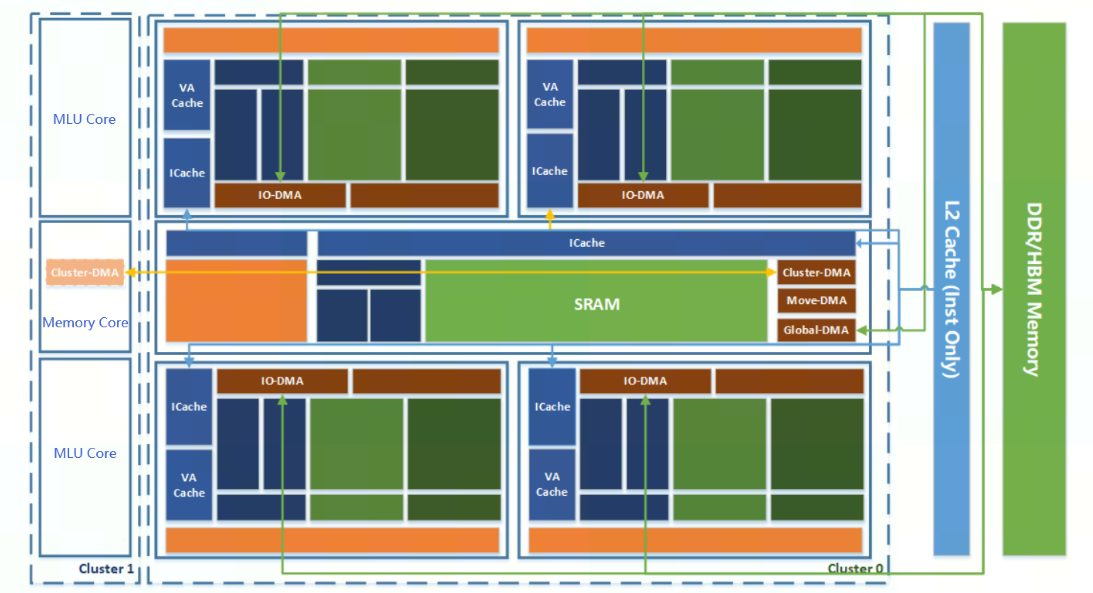
\includegraphics[scale = 0.5]{cluster_arch.png}
    \caption{DLP-M Cluster架构}
    \label{fig:cluster_arch}
    % \note{注:图注的内容不宜放到图题中。}
\end{figure}


\subsection{芯片级优化}

MLU 芯片支持多队列并行,这意味着可以实现多个任务队列并行地执行计算任务及设备端与主机端之间的IO操作。
RT提供了丰富且灵活的队列管理接口、异步 Kernel 执行接口和异步拷贝接口。 使用这些接口
 可以实现硬件资源的高效利用,使得在输入的A维度较大的情况下,可以充分利用 MLU 芯
 片上的 Cluster 计算资源,并行地进行Top-k计算任务, 从而提升算子的并行处理性能。
 假设定义了6个队列,
在实际实现上,首先读取输入,同样设输入规模为[A,B],然后用 A 除以 6,得到每个任务队列至少
  需要处理的输入行数 num\_per\_queue。当 n 不能被 6 整除时, 将余下的待处理
  行从编号为 0 的队列开始,依次加入对应的队列当中,即可得到各队列需要处理的数据。
  接着使用 rtQueueCreate 接口创建好对应的队列,再通过 rtMemcpyAsync 异步
  数据迁移接口将各队列待处理的图像数据 从主机端迁移到设备端。数据迁移完成后即可启
   Kernel 核函数进行 Top-k 算子的计算。最后再次调用 rtMemcpyAsync 异步数据
   迁移接口将计算好的结果从设备端迁移到主机端即可。
通过这样的操作,可以有效的将主机端与设备端之间的IO与计算相互掩盖。达到减少整个任务计算时间的效果,如图~\ref{fig:multi_queue}所示。
\begin{figure}[ht]
    \centering
    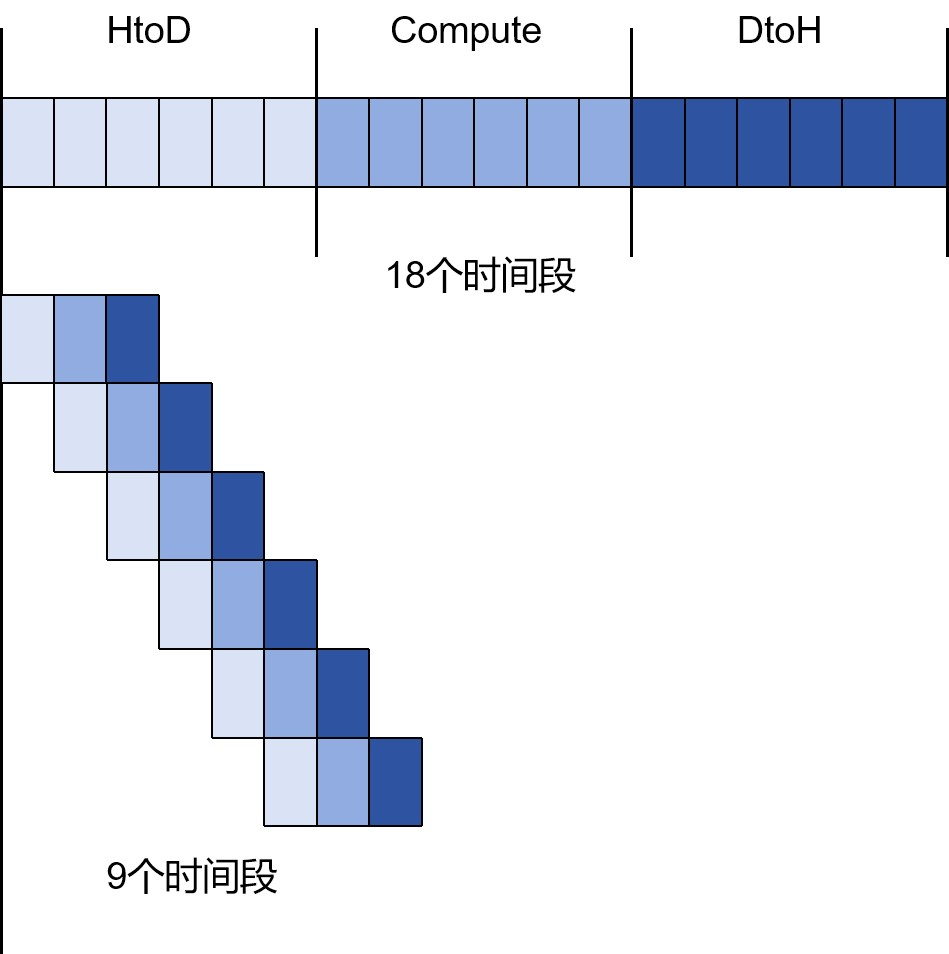
\includegraphics[scale = 0.6]{multi_queue.jpg}
    \caption{多队列优化效果图}
    \label{fig:multi_queue}
    % \note{注:图注的内容不宜放到图题中。}
\end{figure}

\section{本章小结}

本章首先引入了阿姆达尔定律和古斯塔夫森定律,为后续的算子性能优化提供了理论依据,
即提升算子程序的并行度。在此基础上,着重从计算效率和访存效率两个方面对设计实现的 
Top - k 算子进行优化。在计算效率方面,充分利用国产 AI 处理器的硬件资源,
把复杂的计算任务拆分成多个子任务,再合理地分配到各个计算单元。

这种并行处理方式显著提高了 Top - k 算子处理计算任务时的并行度,
进而大幅提升其整体计算效率。同时,通过优化算法计算逻辑、运用融合指令等精细操作,
进一步挖掘处理器的计算潜力,让 Top - k 算子的计算效率得到更进一步提升。
在访存效率方面,围绕减少数据访存量、提高带宽利用率以及实现计算与访存并行化这三大目标,
结合 Top-k 算子计算特点,针对性地采用阶梯化访存、软件流水编排等优化策略。
这些策略不仅有效减少了不必要的数据访存操作,还提高了数据访问的带宽利用率,
使 Top-k 算子在计算过程中能实现计算与访存的良好协同,进一步提升整体性能。









